% This file was created with tikzplotlib v0.10.0.
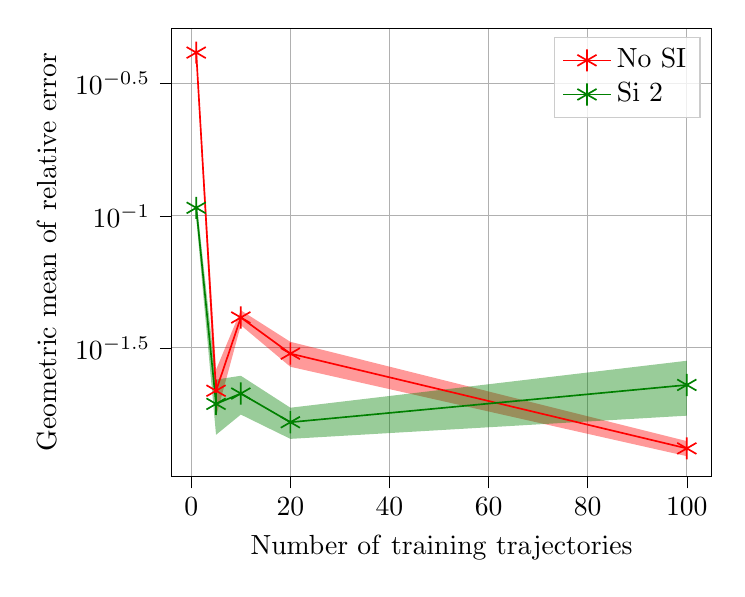
\begin{tikzpicture}

\definecolor{darkgrey176}{RGB}{176,176,176}
\definecolor{green}{RGB}{0,128,0}
\definecolor{lightgrey204}{RGB}{204,204,204}

\begin{axis}[
legend cell align={left},
legend style={fill opacity=0.8, draw opacity=1, text opacity=1, draw=lightgrey204},
log basis y={10},
tick align=outside,
tick pos=left,
x grid style={darkgrey176},
xlabel={\(\displaystyle \mathrm{Number \ of \ training \ trajectories }\)},
xmajorgrids,
xmin=-3.95, xmax=104.95,
xtick style={color=black},
y grid style={darkgrey176},
ylabel={\(\displaystyle \mathrm{Geometric \ mean \ of \ relative \ error }\)},
ymajorgrids,
ymin=0.010309069994386, ymax=0.512910007084145,
ymode=log,
ytick style={color=black}
]
\path [fill=red, fill opacity=0.4, semithick]
(axis cs:1,0.429450303542231)
--(axis cs:1,0.400131225855905)
--(axis cs:5,0.0173958983028854)
--(axis cs:10,0.0385649559314186)
--(axis cs:20,0.026835202131478)
--(axis cs:100,0.0123125426160782)
--(axis cs:100,0.0140391924012675)
--(axis cs:100,0.0140391924012675)
--(axis cs:20,0.0333584891315109)
--(axis cs:10,0.0439005172100248)
--(axis cs:5,0.0261580183317524)
--(axis cs:1,0.429450303542231)
--cycle;

\path [fill=green, fill opacity=0.4, semithick]
(axis cs:1,0.116032739737434)
--(axis cs:1,0.0984242981959792)
--(axis cs:5,0.0148358178207721)
--(axis cs:10,0.0176954549996108)
--(axis cs:20,0.0143181790085377)
--(axis cs:100,0.0175251247780604)
--(axis cs:100,0.0282799080356017)
--(axis cs:100,0.0282799080356017)
--(axis cs:20,0.0187836215621198)
--(axis cs:10,0.0248131332227322)
--(axis cs:5,0.0240010039730088)
--(axis cs:1,0.116032739737434)
--cycle;

\addplot [semithick, red, mark=asterisk, mark size=4, mark options={solid}]
table {%
1 0.414790779352188
5 0.021776957437396
10 0.0412327349185944
20 0.0300968457013369
100 0.013175867497921
};
\addlegendentry{No SI}
\addplot [semithick, green, mark=asterisk, mark size=4, mark options={solid}]
table {%
1 0.107228510081768
5 0.0194184128195047
10 0.0212542954832315
20 0.0165509004145861
100 0.0229025147855282
};
\addlegendentry{Si 2}
\end{axis}

\end{tikzpicture}
